\documentclass[9pt,a4paper,twoside]{tau}
\usepackage[english]{babel}
\usepackage{tauenvs}

%----------------------------------------------------------
% TITLE
%----------------------------------------------------------

\title{Critique of Caterpillar Inc. Stock Report by Josh Feenberg }

%----------------------------------------------------------
% AUTHORS, AFFILIATIONS AND PROFESSOR
%----------------------------------------------------------

\author[a,1]{Bucsa, Justin}

%----------------------------------------------------------

\affil[a]{Stealth}
\professor{}

%----------------------------------------------------------
% FOOTER INFORMATION
%----------------------------------------------------------

\institution{Stealth}
\date{May 2, 2024}
\etal{Bucsa}
\course{}

%----------------------------------------------------------
% ABSTRACT
%----------------------------------------------------------

\begin{abstract}    
    This report critically analyzes the Caterpillar Inc. stock report authored by Josh Feenberg. The analysis dissects each section of Feenberg's report, evaluating its strengths and weaknesses. The critique identifies areas where Feenberg's conclusions are sound and highlights sections requiring further explanation or data analysis to support the claims presented. Finally, the report determines whether Feenberg's overall assessment regarding Caterpillar Inc.'s stock as a long-term and short-term investment is well-founded.
\end{abstract}

%----------------------------------------------------------

\keywords{Caterpillar Inc., critique, stock report}

%----------------------------------------------------------

\begin{document}
		
	\maketitle
	\thispagestyle{firststyle}
	\tauabstract
	\tableofcontents

%----------------------------------------------------------

\section{Introduction}

    This report examines a stock analysis of Caterpillar Inc. conducted by Josh Feenberg. Feenberg utilizes a Jupyter Notebook file to construct a narrative evaluating Caterpillar Inc.'s stock as a potential long-term and short-term investment using two years of historical financial data. 
    
\section{Report Breakdown}

    \subsection{Stock Price}
	
        Feenberg's report, within the "Stock Price" section, accurately observes a significant increase in Caterpillar Inc.'s stock value over the past two years, as evidenced by the provided graph. To strengthen this analysis, Feenberg could quantify the percentage increase in stock value and correlate it to a specific time-frame within the data set.

            \begin{figure}[H]
                \centering
                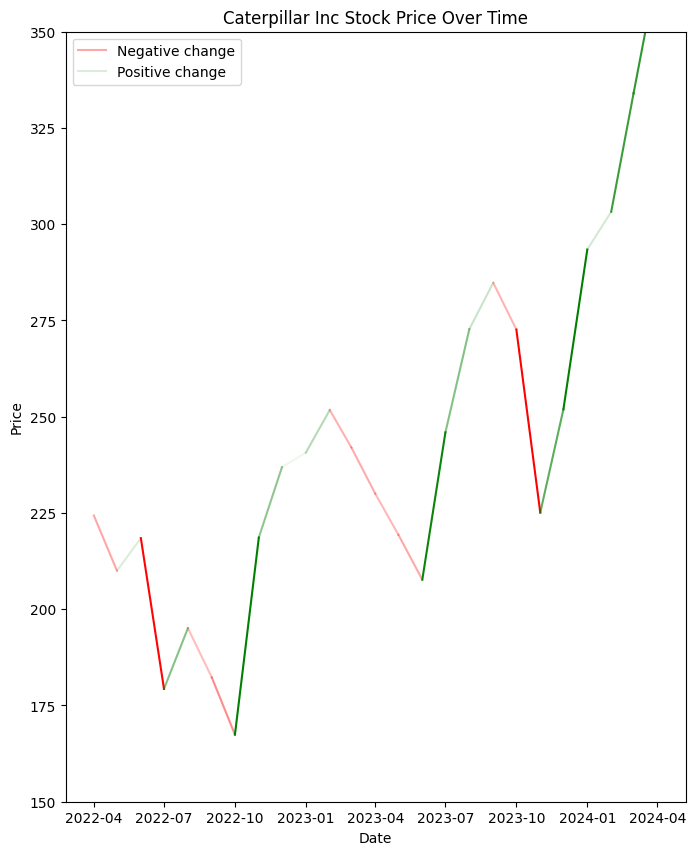
\includegraphics[width=0.8\columnwidth]{CaterpillarIncStockPriceOverTime.png}
                \caption{Caterpillar Inc. stock price over time\cite{feenberg-2024}.} 
                \label {fig:figure}
            \end{figure}

            \subsubsection{Critique}

            Presently, Feenberg's analysis compels the reader to independently identify the cause behind the substantial stock price rise. Ideally, the report should provide a more explanatory narrative to illuminate the factors influencing the price increase.
    
    \subsection{Volume}

        The "Volume" section of the report acknowledges a recent decline in the volume of stock traded. Feenberg attributes this decrease to the preceding price surge, suggesting that investors are adopting a wait-and-see approach before resuming typical trading patterns as the stock price stabilizes. This aligns with market behavior.
 
            \begin{figure}[H]
                \centering
                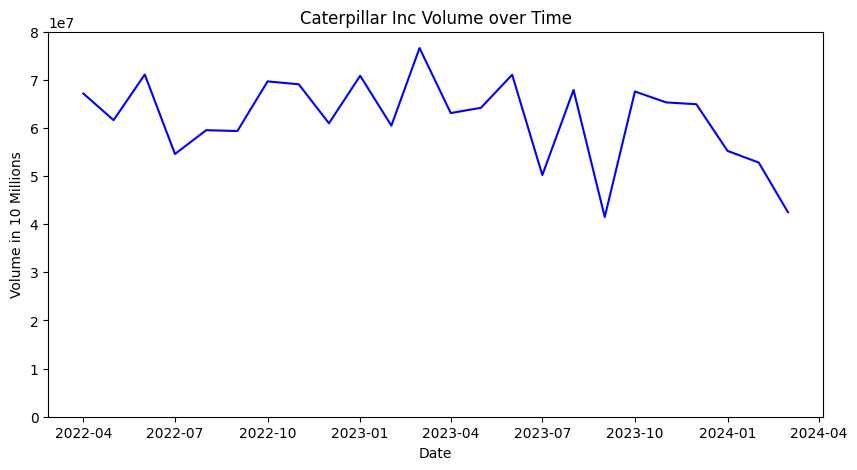
\includegraphics[width=0.8\columnwidth]{CaterpillarIncVolumeOverTime.png}
                \caption{Caterpillar Inc volume over time\cite{feenberg-2024}.}
                \ref{fig:figure}
            \end{figure}

            \subsubsection{Critique}

            While Feenberg identifies a key factor influencing the recent decline in trading volume, the explanation can be further enhanced. Juxtaposing corresponding graphs from the "Stock Price" and "Volume" sections would provide a visual aid, strengthening the comprehension of Feenberg's observations.

    \subsection{Earnings}    

        Feenberg analyzes the company's earnings report for the past two years and asserts that it does not correspond to the stock price increase.
        
            \begin{figure}[H]
                \centering
                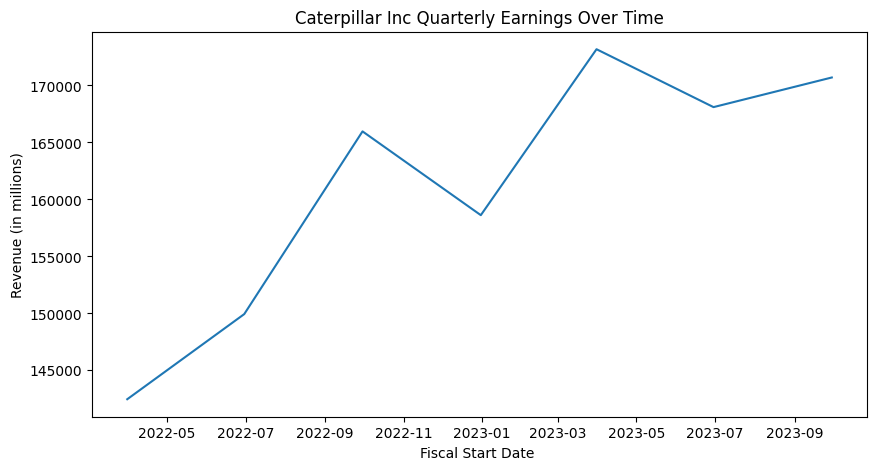
\includegraphics[width=0.8\columnwidth]{CaterpillarIncQuarterlyEarningsOverTime.png}
                \caption{Caterpillar Inc. quarterly earnings over time\cite{feenberg-2024}.} 
                \ref{fig:figure}
            \end{figure}

            \subsubsection{Critique}

                Feenberg's critique regarding the earnings report requires further elaboration. A closer examination reveals that the earnings report exhibits fluctuations similar to the stock price, albeit with a potential time lag. This suggests that the earnings report might be predictive of future stock value. 

    \subsection{Major Events in Last Two Years}  

        This section identifies three significant developments at Caterpillar Inc. within the past two years:
        
            \begin{enumerate}
                \item {Appointment of Joseph E. Creed as Chief Operating Officer in October 2023\cite{feenberg-2024}.}
                \item {Appointment of Jason Kaiser as President of the New Energy and Transportation Group in January 2024\cite{feenberg-2024}.}
                \item {Demonstration of Caterpillar Inc.'s new sustainable underground mining technology to Newmont\cite{feenberg-2024}.}
            \end{enumerate}

            \subsubsection{Critique}

                While these events might be considered pivotal moments in Caterpillar Inc.'s recent history, Feenberg does not investigate whether they impacted the stock price. The report leaves the reader to determine their potential significance.

    \subsection{Dominant Shareholders of Company}

        This section details the dominant shareholders of Caterpillar Inc. and their ownership percentages:
            \begin{enumerate}
                \item{Institutional investors hold 72\% of the company's stock\cite{feenberg-2024}.}
                \item{The Vanguard Group holds 9.7\% of the total stock \cite{feenberg-2024}.}
                \item{ Board members and top-level management own less than 1\% of the total stock, valued at approximately \$312 million\cite{feenberg-2024}.}
                \item{The general public owns the remaining 28\% of the total stock\cite{feenberg-2024}.}  
            \end{enumerate}

            \subsubsection{Critique}

                Understanding the distribution of ownership in Caterpillar Inc. is valuable. However, Feenberg neglects to analyze how this ownership structure might influence the stock price.
                
    \subsection{Goal and Philosophy of the Company}

        Feenberg cites Caterpillar Inc.'s website to state the company's primary goals as "sustainable development and innovation"\cite{feenberg-2024}.

            \subsubsection{Critique}

                Feenberg omits a crucial element –  evidence substantiating this stated goal as Caterpillar Inc.'s genuine focus. Ideally, the report should leverage past/current/future events, investments, or data to demonstrate the company's commitment to these goals. 

\section{Agreeable Findings}

    Feenberg's observation in the "Volume" section regarding the current trading volume aligns with market behavior. The decline in trading volume can be attributed to investors waiting for the stock price to stabilize following the recent surge. 

\section{Disagreeable Findings}    

    Feenberg's conclusion regarding the earnings report requires further analysis. A closer examination reveals that the earnings report exhibits fluctuations similar to the stock price, albeit with a potential time lag. This suggests that the earnings report might be a leading indicator of future stock value. The earnings may not directly reflect the current stock price, but they could foreshadow its trajectory in the coming quarters.


\section{Rationality of the Report}

    Feenberg's report suffers from brevity, hindering its ability to reach a definitive conclusion regarding Caterpillar Inc. stock as a viable investment. While the data utilized appears accurate and holds promise, the analysis lacks depth and requires further explanation to support the claims presented. Feenberg would benefit from including additional explanations alongside the data to strengthen the report's rationale. 

\section{Conclusion}
    This report provides a critical analysis of Josh Feenberg's stock report on Caterpillar Inc. The critique identifies areas where Feenberg's observations are sound and highlights sections requiring further investigation. While Feenberg utilizes accurate data, the report would be strengthened by including a more thorough analysis with additional explanations to support the conclusions drawn.

    Overall, Feenberg's report offers a valuable starting point for understanding Caterpillar Inc.'s stock, but further research is needed to determine its suitability as a long-term or short-term investment.


        
%----------------------------------------------------------

\addcontentsline{toc}{section}{References}
\printbibliography

%----------------------------------------------------------

\begin{center}
	\vskip10pt
	% Enjoy writing with tau \LaTeX\ class $\blacksmiley$ \\ 
	\vskip10pt
	\textit{Contact:} \\
	% \faLink\ \href{https://sites.google.com/view/memo-notess/p%C3%A1gina-principal}{https://sites.google.com/memo-notess} \\
	\faEnvelope[regular]\ justin.bucsa@gmail.com \\
	% \faInstagram\ memo.notess\\
\end{center}


%----------------------------------------------------------

\end{document}